\section{Task: Ghost cells exchange between neighboring processes [15 Points]}
For this exercise we create a Cartesian communicator with periodic boundaries, in order to find the neighboring ranks using the \texttt{MPI\_Cart\_Shift} function.
After finding all four neighbors we do four \texttt{MPI\_Sendrecv} executions, where each processes, for example receives the values from the southern neighbor and sends its values to the northern neighbor, which is then repeated for each direction. Note that this is possible because we have periodic boundaries which means every processes has a neighbor in every direction.
\begin{lstlisting}[language=C++, caption=Example, label=lst:sendrc]
// Create cartesian topology
MPI_Cart_create(MPI_COMM_WORLD, 2, dims, periods, 1, &comm_cart);

// Finding neighbors
MPI_Cart_shift(comm_cart, 0, 1, &rank_top, &rank_bottom);
MPI_Cart_shift(comm_cart, 1, 1, &rank_left, &rank_right);

// Send values to northern neighbor and receive from southern neighbor
MPI_Sendrecv(&data[1 * DOMAINSIZE + 1], 1, T_row, rank_top, 0,
		   &data[(SUBDOMAIN + 1) * DOMAINSIZE + 1], 1, T_row, rank_bottom,
		   0, comm_cart, MPI_STATUS_IGNORE);

/* REPEATED FOR EACH DIRECTION */
\end{lstlisting}
In order to simply the communications, we introduce two new MPI data types. For the row we define a \texttt{MPI\_Type\_contiguous}, which is simply for values that are stored in a contiguous location. For the columns we define \texttt{MPI\_Type\_vector} data types, which allows us to define a stride and therefore columns in a contiguous stored matrix.
\begin{lstlisting}[language=C++, caption=Example, label=lst:mpi_type]
MPI_Datatype T_row, T_col;
MPI_Type_contiguous(SUBDOMAIN, MPI_DOUBLE, &T_row);
MPI_Type_vector(SUBDOMAIN, 1, DOMAINSIZE, MPI_DOUBLE, &T_col);
MPI_Type_commit(&T_col);
MPI_Type_commit(&T_row);
\end{lstlisting}
For the exchange of ghost cells of the neighbors in ordinal direction, we use the \texttt{MPI\_Cart\_coords} function, which returns the coordinates of a process in a communicator of a cartesian topology. By adding $+1$ or $-1$ to its own x and y coordinates, a process can figure out its ordinal neighbors as seen in Listing \ref{lst:ordinal}. Finally we do a send and receive similarly as before, just in ordinal direction. For example sending the value to the northeast and receiving the values from southwest.
\begin{lstlisting}[language=C++, caption=Example, label=lst:ordinal]
int top_right_rank, top_left_rank, bottom_right_rank, bottom_left_rank;
int top_right_coords[2] = {coords[0] - 1, coords[1] + 1};
MPI_Cart_rank(comm_cart, top_right_coords, &top_right_rank);
int top_left_coords[2] = {coords[0] - 1, coords[1] - 1};
MPI_Cart_rank(comm_cart, top_left_coords, &top_left_rank);
int bottom_right_coords[2] = {coords[0] + 1, coords[1] + 1};
MPI_Cart_rank(comm_cart, bottom_right_coords, &bottom_right_rank);
int bottom_left_coords[2] = {coords[0] + 1, coords[1] - 1};
MPI_Cart_rank(comm_cart, bottom_left_coords, &bottom_left_rank);

// Send top right and receive from bottom left
MPI_Sendrecv(&data[1 * DOMAINSIZE + (DOMAINSIZE - 2)], 1, MPI_DOUBLE,
               top_right_rank, 0, &data[(DOMAINSIZE - 1) * DOMAINSIZE + 0], 1,
               MPI_DOUBLE, bottom_left_rank, 0, comm_cart, MPI_STATUS_IGNORE);

/* REPEATED FOR EVERY ORDINAL DIRECTION */
\end{lstlisting}

\begin{figure}[H]
	\centering
	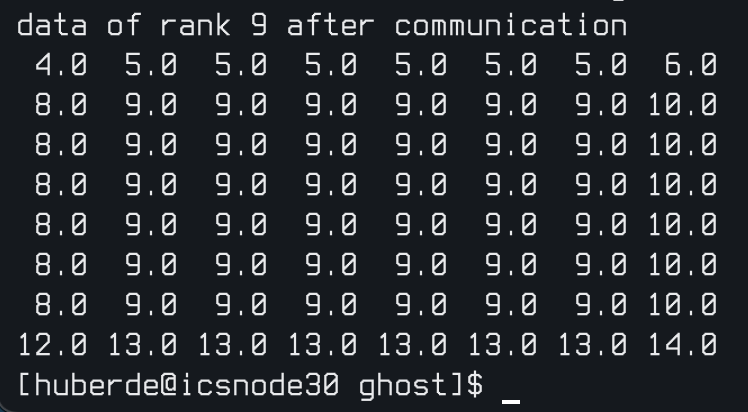
\includegraphics[width=0.5\textwidth]{../media/ghost.png}
	\caption{Result for process with Rank 9}
	\label{fig:dgemm-fm}
\end{figure}


